
This work depends on three factors; both static and motion information
are vital for action recognition, but the final accuracy depends on the ratio of contribution of each domain,
and the optimum contribution may depend on the data set. We derive our fusion models addressing all these aspects.
The three mathematical models we used
to fuse the static and motion vectors are described next. This sub section relates to the ``Fusion layer'' block in Fig. \ref{fi:overall}.

\subsubsection{Cholesky Transformation Based Method}

This derivation is based on the Cholesky transformation. An
abstract version of Cholesky transformation is described below.

Let $P$ and $Q$ be two random variables of unknown correlation. These random variables can be
transformed into two new random variables ($R$ and $S$) with a known correlation of $\rho$, where the
value of $\rho$ can be chosen at will. The transformation can be performed as follows.

\begin{equation}
\begin{bmatrix}
    Y     \\
    Z
\end{bmatrix}
=
\begin{bmatrix}
    1  & 0 \\
    \rho  & \sqrt{1-\rho^2}
\end{bmatrix}
\times
\begin{bmatrix}
    P     \\
    Q
\end{bmatrix}
\end{equation}

Therefore,

\begin{equation}
Y = P
\end{equation}

and

\begin{equation}
Z = \rho P + \sqrt{1-\rho^2}Q
\end{equation}

The Cholesky transformation guarantees that the correlation between the two random variables
$Y$ and $Z$ is $\rho$.

Based on the above properties of the Cholesky transformation, we propose the following methodology to fuse the static and motion vectors.

Let $S$ and $M$ be static and motion vectors, respectively. Cholesky transformation can be applied to the two vectors $S$ and $M$ with the correlation value $\rho_{1}$.

\begin{equation}
\begin{bmatrix}
    Y     \\
    Z
\end{bmatrix}
=
\begin{bmatrix}
    1  & 0 \\
    \rho_{1}  & \sqrt{1-\rho_{1}^2}
\end{bmatrix}
\times
\begin{bmatrix}
    S    \\
    M
\end{bmatrix}
\end{equation}

\begin{equation}
Y = S
\end{equation}

\begin{equation}
Z = \rho_{1} M + \sqrt{1-\rho_{1}^2}M
\end{equation}

Similarly, the transformation can be applied to $M$ and $S$ with the correlation value $\rho_{2}$.


\begin{equation}
\begin{bmatrix}
    A     \\
    B
\end{bmatrix}
=
\begin{bmatrix}
    1  & 0 \\
    \rho_{2}  & \sqrt{1-\rho_{2}^2}
\end{bmatrix}
\times
\begin{bmatrix}
    M    \\
    S
\end{bmatrix}
\end{equation}

\begin{equation}
A = M
\end{equation}

\begin{equation}
B = \rho_{2} S + \sqrt{1-\rho_{2}^2}S
\end{equation}

Again, the Cholesky transformation guarantees the following two properties.


\begin{enumerate}
  \item The correlation between $S$ and $Z$ is $\rho_{1}$.
  \item The correlation between $M$ and $B$ is $\rho_{2}$.
\end{enumerate}

Therefore, if the values of $\rho_{1}$ and $\rho_{2}$ are chosen in such a way that they obey the following
rule,

\begin{equation}
\rho_{2} = \sqrt{1-\rho_{1}^2}
\end{equation}

it can be guaranteed that $Z = B$, $\forall S,M,\rho_{1},\rho_{2}$. Hence, the resultant vector $C$ can be obtained
by,

\begin{equation}
C=Z=B
\end{equation}

where the correlation between $C$ and $S$ is $\rho_{1}$ and the correlation between $C$ and $M$ is $\rho_{1}$. Here $S$ and $M$ represent the static and the
motion vectors whereas $C$ represents the resultant vector. This derivation
leads us to an important intuition: by choosing the value of $\rho_{1}$, we can
choose the degree to which the static features and the motion features contribute,
in deriving the resultant vector. In section 4, it is shown, how this property is used to explore, the optimal contribution of
static and motion domain information for recognizing actions.

\subsubsection{Variance Ratio Based Method}

The second method employed to combine the motion and static vectors is based on a Gaussian probability model. We model each vector as a histogram. Further, we assume the two vectors are independent to each other. Using the histogram model, the mean and variance of each vector are calculated in order to fit the two vectors into Gaussian distributions. The joint Gaussian distribution is then computed based on this data.

\begin{equation}
G_{sm}= \frac{1}{2\pi\sigma_m\sigma_s} e^{-\left[\frac{[N-\mu_s]^2}{2\sigma_s^2}+ \frac{[N-\mu_m]^2}{2\sigma_m^2} \right]}
\end{equation}

This computation corresponds to the evaluation line obtained when equating the two random variables as shown below. The combined distribution is then be obtained through this process.

It must be noted that both histograms (corresponding to static and motion components) do not contain equal information. Hence varying the contribution of each histogram to the resultant distribution is necessary. This requires varying of the evaluation line which can be achieved through scaling of the motion and static axes. This scaling process is carried out by the following matrix.


\[
\begin{bmatrix}
    \frac {\sigma_s}{\sigma_s + \sigma_m} & 0  \\
    0 & \frac {\sigma_m}{\sigma_s + \sigma_m}
\end{bmatrix}
\]

We may conclude that higher variance of a component along one axis reflects lower detail in the model with regards to the other axis. Considering the motion axis, the contribution of the static vector towards the resultant vector may be defined by $(1-\frac{\sigma_m}{\sigma_m+\sigma_s})$. A high variance always corresponds to a flatter histogram containing less detail.

This parameter we derive is significant as it defines the contribution of each individual motion and static vector pair independent of explicit terms. Hence the optimum ratio for combination of motion and static components of a given data set can be mathematically evaluated. With regards to the data sets used for experimenting, 30\% of motion
vector and 70\% of static vector constitute this parameter on average. This mathematical inference is further verified through the experiment results in section IV.

Defining new parameters $N_s$ and $N_s$ as follows, we build a new distribution which is a scaled version of the joint Gaussian distribution obtained previously.

\begin{align*}
N_s &= N \frac{\sigma_m}{\sigma_m+\sigma_s}  \\
N_s &= N \frac{\sigma_s}{\sigma_m+\sigma_s}
\end{align*}

Dropping our initial assumption of independence between the motion and static vectors, we define the following distribution representative of the combined vector.

\begin{equation}
G_{sm}= \frac{e^{-\frac{1}{2(1-\rho^2)}\left[\frac{[N_s-\mu_s']^2}{2\sigma_s'^2} + \frac{[N_m-\mu_m']^2}{2\sigma_m'^2} - \frac{2\rho[N_s-\mu_s'][N_m-\mu_m']}{\sigma_s' \sigma_m'}  \right]}}{2\pi\sigma_m'\sigma_s'\sqrt{1-\rho^2}}
\end{equation}

\subsubsection{PCA Based Method}

The third fusion method is based on Principle Component Analysis (PCA). PCA is a statistical procedure that uses an orthogonal transformation to convert a
set of observations of possibly correlated variables into a set of values of linearly uncorrelated
variables called principal components. This transformation is defined in such a way that the first
principal component has the largest possible variance (that it accounts for as much of the
variability in the data as possible), and each succeeding component in turn has the highest
variance possible under the constraint that it is orthogonal to the preceding components. The
resulting vectors are an uncorrelated orthogonal basis set.

If there are $n$ number of features in the input vector of the PCA, the output of the
PCA will provide a new set of $n$ features which are orthogonal and uncorrelated. Also, if
$\mathrm{output} =[a_{1}, a_{2}, ..., a_{n}]$, then $\mathrm{var}(a_{1})> \mathrm{var}(a_{2})> \dots > \mathrm{var} (a_{n})$.
Due to the properties of the PCA, the original set of n features can be
represented precisely using the first $k (n>k)$ principal
components of the output vector, given that the total squared reconstruction error
is minimized.

In other words, the essence of the original $n$ dimensional data set is now almost
completely represented by the new $k$ dimensional data set with a minor data loss. Thus, the
dimension of the data set is reduced from $n$ to $k$.


In our work, the dimensionality of the data set $T$ is 2 (number of feature domains: static
and motion).
Using PCA on $T$, we receive a new set $T$', with 2 new features domains. We need only one new feature
domain in the feature space to
represent motion and static domains. Therefore, it is our aim to extract only the first principal component.
In order to do this, we need to justify that the first principal component contains a significant majority of
the essence of the original data set. In other words, only a negligible amount of data is lost by
eliminating the second principal component.

Therefore, we perform PCA on over 15,000 samples of motion and static
vectors and plot the variance percentage of the total variance
explained by the first and the second principal components respectively, as in figure and figure


It is evident from the figure that the first principal component almost always accounts
for over 97\% of the essence of the original data set, except for only a negligible amount
of samples. The lowest percentage registered is approximately 85\%, which is still a
significantly high value. Figure \ref{fi:pca} shows the percent standard deviation values for the first and second components of the PCA for the two data sets.

\begin{figure}
  \centering
  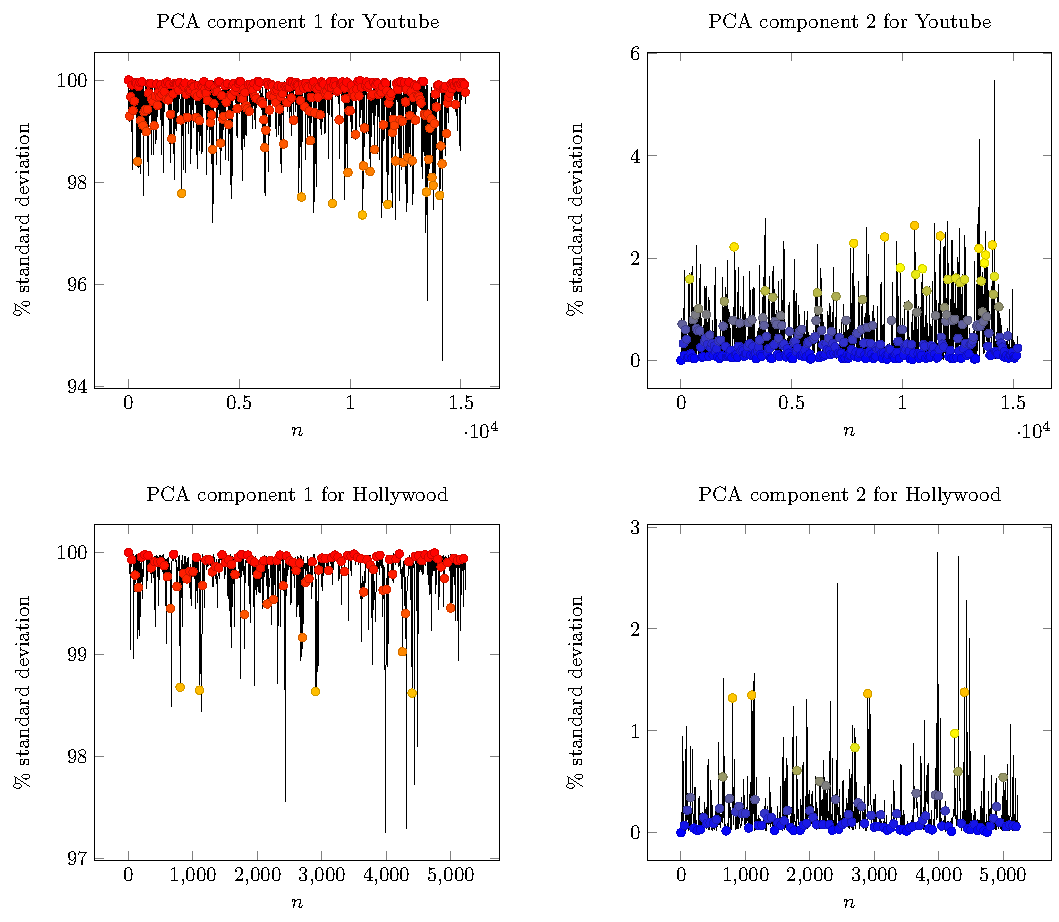
\includegraphics[width=3.5in]{figures/pca.pdf}
  \caption{Percent standard deviation values for the first and second components of the PCA. $n$ is the feature vector index. }\label{fi:pca}
\end{figure}


Therefore, by eliminating the second principal component, only less than 5\% of data
is lost in average, and hence only the first principal component can be used to accurately
represent the original data set. 